% Patron de document pour un article a JFSMA pour LaTeX 2e
% Copyright (c) 2007 Bruno BEAUFILS
% Les quolibets et autres insultes sont à envoyer à bruno.beaufils@univ-lille.fr
% Modifications par Gauthier Picard (gauthier.picard@onera.fr) - 31-mai-07
% Modifications par Pierre Chevaillier (chevaillier@enib.fr) - 20-mar-2007
% Modifications par Yann Krupa (krupa@emse.fr) et Gauthier Picard (gauthier.picard@onera.fr) - 31-mar-2011
% Modifications par Emmanuel Adam (emmanuel.adam@univ-valenciennes.fr) - 31-mar-2011
% Modifications par Gauthier Picard (gauthier.picard@onera.fr) - 16-nov-2014
% Modifications par Gauthier Picard (gauthier.picard@onera.fr) - 29-nov-2017
% Modifications mineures par Maxime Morge (maxime.morge@univ-lille.fr) - 3-nov-2023
% L'option doit être :
% - contribution, pour une contribution scientifique originale
% - dissemination, pour une contribution scientifique déjà publiée mais
% inédite en français et traduite ici
% - sota, pour un état de l'art
% - demonstration, pour un article support à démonstration de logiciels
% - final, pour la version finale
\documentclass[dissemination]{jfsma}

% --- Tickz
\usepackage{physics}
\usepackage{tikz}
\usepackage{amsmath}
\usepackage{mathdots}
% \usepackage{yhmath}
\usepackage{cancel}
\usepackage{color}
\usepackage{siunitx}
\usepackage{array}
\usepackage{multirow}
% \usepackage{amssymb}
\usepackage{gensymb}
\usepackage{tabularx}
\usepackage{extarrows}
\usepackage{booktabs}
\usetikzlibrary{fadings}
\usetikzlibrary{patterns}
\usetikzlibrary{shadows.blur}
\usetikzlibrary{shapes}
% ---------

\usepackage{amssymb}
\usepackage{csquotes}
\usepackage[export]{adjustbox}

\usepackage{tabularray}\UseTblrLibrary{varwidth}
\usepackage{xcolor}
\def\BibTeX{{\rm B\kern-.05em{\sc i\kern-.025em b}\kern-.08em
    T\kern-.1667em\lower.7ex\hbox{E}\kern-.125emX}}
\usepackage{amsmath}
\newcommand{\probP}{\text{I\kern-0.15em P}}

\newcommand{\myCustomSize}[1]{%
  \fontsize{9}{10.8}\selectfont
  #1
}

\DeclareMathAlphabet\mathbfcal{OMS}{cmsy}{b}{n}

\titre{Une approche organisationnelle pour améliorer l’explicabilité et le contrôle dans l’apprentissage par renforcement multi-agent}


\auteur{Julien Soulé\up{a,b}}{julien.soule@lcis.grenoble-inp.fr}
\auteur{Jean-Paul Jamont\up{a}}{jean-paul.jamont@lcis.grenoble-inp.fr}
\auteur{Michel Occello\up{a}}{michel.occello@lcis.grenoble-inp.fr}
%%%Si besoin d'ajouter des auteurs à la ligne :
\auteurSuite{Louis-Marie Traonouez\up{b}}{louis-marie.traonouez@thalesgroup.com}
\auteurSuite{Paul Théron\up{c}}{paul.theron@orange.fr}

\institution{\up{a}%
  Univ. Grenoble Alpes, Grenoble INP, LCIS, 26000, Valence, France}
\institution{\up{b}%
  Thales Land and Air Systems, BU IAS, Rennes, France}
\institution{\up{c}%
  AICA IWG, La Guillermie, France}

\begin{document}

\maketitle

\begin{resume}
  L'apprentissage par renforcement multi-agent (MARL) peut faire émérger des comportements collaboratifs s'apparentant à une organisation. Nous proposons le cadre MOISE+MARL pour faire évoluer explicitement les agents de façon organisationelle. En attribuant des rôles et des objectifs aux agents, MOISE+MARL contrôle l'apprentissage en ajustant les actions et les récompenses. De plus, il propose une analyse post-entraînement pour inférer des spécifications organisationnelles implicites.
  MOISE+MARL est appliqué dans divers environnements et d'algorithmes, montrant un alignement des agents aux spécifications organisationnelles prédéfinies, lesquelles correspondent à celles déduites.
\end{resume}

\motscles{Apprentissage par renforcement multi-agent, Explicabilité organisationnelle, Contrôle organisationnel}

% \bigskip

\begin{abstract}
  Multi-Agent Reinforcement Learning (MARL) can give rise to collaborative behaviors resembling an organization. We introduce the MOISE+MARL framework to explicitly make agents evolve in an organizational manner. By assigning roles and objectives to agents, MOISE+MARL controls the learning process by adjusting actions and rewards. Moreover, it includes a post-training analysis to infer implicit organizational specifications.
  MOISE+MARL has been applied to various environments and algorithms, demonstrating an alignment between trained agents and predefined organizational specifications, which match the inferred ones.
\end{abstract}
\keywords{Multi-Agent Reinforcement Learning, Organizational Explainability, Organizational Control}


\section{Introduction}

% Contexte  
L'apprentissage par renforcement multi-agent (MARL) permet de trouver une politique conjointe qui régit à la fois les actions individuelles et les interactions entre agents pour atteindre un objectif sans gérer leur coordination explicitement. Dans des environnements nécéssitant des interactions sociales, les agents peuvent parfois aboutir à des comportements semblables à des rôles et objectifs implicites, qui les rapprochent, dans une certaine mesure, d'une organisation structurelle et fonctionnelle théorique, telle que décrite dans $\mathcal{M}OISE^+$~\cite{Hubner2007}.


% Problématique  
Nous définissons l'\textbf{adéquation organisationnelle} comme la mesure de la similitude entre les comportements réels des agents et une organisation structurelle et fonctionnelle. Deux aspects clés sont alors à explorer :
i) \textbf{L'évaluation de l'adéquation organisationnelle} consiste à mesurer l'alignement d'une politique conjointe avec une organisation idéale, en tenant compte des contraintes environnementales et des objectifs. La littérature, souvent centrée sur les rôles ou objectifs~\cite{Isakov2024, Wen2024, Xie2024}, manque d'approches systématiques dotées de moyens quantitatifs ou qualitatifs
 ; \quad
ii) \textbf{Le contrôle de l'adéquation organisationnelle} consiste à orienter les agents vers des politiques conformes à une organisation via des contraintes ou incitations définies par l'utilisateur. Ce contrôle induit la réduction de l'espace de recherche, l'amélioration de la convergence et le respect des contraintes de sécurité, sans recourir à l'apprentissage par renforcement hiérarchique (HRL).


% Contribution  
\noindent Cet article présente le cadre \textbf{MOISE+MARL} que nous avons introduit dans \cite{soule2025moisemarl}. MOISE+MARL apporte une contribution synthétique en simplfiant la complexité des premiers travaux sur l'intégration d'un modèle organisationnel dans le MARL~\cite{soule2024paper-jfsma, soule2024aomea} en se recentrant sur la notion de rôles et objectifs, permettant une meilleure utilisabilité et scalabilité. Il combine le Dec-POMDP et le modèle organisationnel $\mathcal{M}OISE^+$~\cite{Hubner2007} via des relations définies, permettant aux utilisateurs de spécifier la logique des rôles et objectifs à partir de motifs de trajectoires. Une fois configuré, le cadre attribue des rôles aux agents en imposant des contraintes qui ajustent dynamiquement l'espace d'actions et la fonction de récompense. Il intègre également la méthode \textit{Trajectory-based Evaluation in MOISE+MARL} (TEMM), qui, par apprentissage non supervisé, infère les rôles et missions implicites à partir de trajectoires observées, offrant ainsi une évaluation quantitative de l'adéquation organisationnelle. Contrairement au HRL, qui décompose les tâches~\cite{Qi2024, Matsuyama2025, SaoMai2024}, notre approche guide les agents par des rôles et des missions explicites.

% Évaluation et résultats  
Nous avons évalué MOISE+MARL avec :
i) Quatre environnements différents, chacun entraînant des politiques nécéssitant des organisations implicites variées, afin d'évaluer la généralisabilité du cadre
 ; \quad
ii) Quatre algorithmes MARL de familles distinctes, pour mesurer leur adéquation avec MOISE+MARL lors de l'entraînement et de l'analyse post-entraînement
 ; \quad
iii) Un ensemble de spécifications organisationnelles par environment, permettant une évaluation manuelle et quantitative de leurs impacts.
%
Une observation manuelle montre qu'un agent adoptant un rôle et engagé dans une mission, s'aligne effectivement sur le comportement attendu, confirmant la mesure de l'adéquation organisationnelle obtenue via TEMM. Les rôles et missions inférés s'alignent sur les spécifications prédéfinies, démontrant la cohérence interne du cadre. Par ailleurs, les algorithmes basés sur la politique et les actor-critic produisent des politiques stables, tandis que ceux basés sur la valeur présentent une variabilité plus importante.


% Structure de l'article  
\noindent La \autoref{sec:related_works} présente les travaux sur l'adéquation organisationnelle, la \autoref{sec:moise_marl_framework} introduit MOISE+MARL, la \autoref{sec:TEMM_algorithm} décrit TEMM, la \autoref{sec:experimental_setup} expose le protocole expérimental et la \autoref{sec:results} les résultats, puis la \autoref{sec:discussion_conclusion_future_work} conclut.

\section{Travaux connexes}
\label{sec:related_works}

Cette section explore des travaux liées aux deux aspects de l'adéquation organisationnelle.

\subsection{Évaluation de l'adéquation organisationnelle}

Certains travaux se sont intéressés à l'inférence de rôles ou d'objectifs pour mesurer l'adéquation organisationnelle ou des concepts similaires.  
%
Wilson et al.~\cite{wilson2008learning} proposent un transfert de rôles dans les MDPs multi-agent pour faciliter l'adaptation entre environnements, mais leur modèle se limite à des rôles spécifiques liés aux tâches.  
%
Berenji et Vengerov~\cite{berenji2000learning} étudient la coordination et l'inférence de rôles dans des missions \textit{Unmanned Aerial Vehicles} pour renforcer la coopération, sans permettre d'inférer les rôles implicites requis.  
%
Yusuf et Baber~\cite{yusuf2020inferential} utilisent des méthodes bayésiennes pour coordonner des agents diversifiés, mais leur approche manque d'abstraction des rôles et n'évalue pas l'alignement avec une structure organisationnelle globale.  
%
Serrino et al.~\cite{serrino2019finding} explorent l'inférence dynamique des rôles dans des environnements sociaux, se concentrant sur des rôles opérationnels immédiats plutôt que sur des rôles implicites.

Tous les travaux identifiés intègrent des mécanismes internes impliquant une inférence \textquote{faite-main} ou manipulation implicite des rôles pour servir une coordination global. MOISE+MARL se concentre seulement sur l'explicitation des rôles et objectifs de façon général et la mesure quantitative de l'adéquation organisationelle.

\subsection{Contrôle de l'adéquation organisationnelle}

Le contrôle de l'adéquation organisationnelle consiste à aligner les politiques des agents sur une organisation prédéfinie via des contraintes ou incitations. Par exemple, Achiam et al.~\cite{achiam2017cpo} présentent le \textit{Constrained Policy Optimization} (CPO), qui ajuste les politiques avec des contraintes de sécurité tandis que MOISE+MARL va plus loin en appliquant des contraintes externes qui modifient dynamiquement l'espace d'action pour orienter les agents vers des comportements organisationnels.

Ray et al.~\cite{ray2019benchmarking} intègrent des contraintes dans la fonction de récompense via des multiplicateurs de Lagrange. MOISE+MARL étend cette approche en imposant des contraintes à divers niveaux pour offrir un contrôle flexible. De même, alors que Garcia et al.~\cite{garcia2015comprehensive} et Alshiekh et al.~\cite{alshiekh2018safe} se concentrent sur l'exploration sécurisée, MOISE+MARL guide les agents vers des comportements alignés avec des rôles.

Plutôt que de décomposer les tâches en sous-tâches comme le HRL~\cite{ghavamzadeh2006hrl}, MOISE+MARL contraint le MARL de manière externe, assurant une granularité modulaire et des comportements affinés. Enfin, la coordination décentralisée par partage des connaissances~\cite{foerster2018communication} illustre l'importance d'une communication maîtrisée pour garantir l'adéquation organisationnelle dans les systèmes complexes.

MOISE+MARL se distingue en intégrant des contraintes organisationnelles externes dans un cadre MARL standard, modifiant actions et récompenses pour aligner les comportements sur des rôles, contrairement aux approches classiques telles que le shielding ou le CPO.


\section{Le cadre MOISE+MARL}
\label{sec:moise_marl_framework}

Cette section présente le formalisme utilisé pour décrire le cadre MOISE+MARL.

\subsection{Cadre de Markov pour le MARL}

Pour appliquer les techniques de MARL, nous nous appuyons sur le \textit{Decentralized Partially Observable Markov Decision Process} (Dec-POMDP)~\cite{Oliehoek2016}. Les Dec-POMDP modélisent naturellement la coordination décentralisée multi-agent en situation d'observabilité partielle, ce qui les rend particulièrement adaptés à l'intégration de contraintes organisationnelles. Contrairement aux \textit{Partially Observable Stochastic Games} (POSG), le Dec-POMDP comprend une fonction de récompense commune, favorisant ainsi la collaboration~\cite{Beynier2013}.

Un Dec-POMDP $d \in D$ (où $D$ est l'ensemble des Dec-POMDP) est défini comme un 7-uplet 
$d = \langle S, \{A_i\}, T, R, \{\Omega_i\}, O, \gamma \rangle$,
où 
\(S = \{s_1,\dots,s_{|S|}\}\) est l'ensemble des états possibles ; \quad
\(A_i = \{a_{1}^{i},\dots,a_{|A_i|}^{i}\}\) est l'ensemble des actions possibles pour l'agent \(i\) ; \quad
\(T\) représente l'ensemble des probabilités de transition, avec \(T(s,a,s') = \probP(s'|s,a)\) qui correspond à la probabilité de passer de l'état \(s\) à l'état \(s'\) suite à l'action \(a\) ; \quad
\(R : S \times A \times S \rightarrow \mathbb{R}\) est la fonction de récompense, attribuant une récompense en fonction de l'état initial, de l'action effectuée et de l'état résultant ; \quad
\(\Omega_i = \{o_{1}^{i},\dots,o_{|\Omega_i|}^{i}\}\) est l'ensemble des observations possibles pour l'agent \(i\) ; \quad
\(O\) représente l'ensemble des probabilités d'observation, où \(O(s',a,o) = \probP(o|s',a)\) est la probabilité d'obtenir l'observation \(o\) après avoir effectué l'action \(a\) et atteint l'état \(s'\) ; \quad et enfin, \(\gamma \in [0,1]\) est le facteur d'actualisation.

Le formalisme suivant est utilisé avec MOISE+MARL pour résoudre le Dec-POMDP~\cite{Beynier2013,Albrecht2024} :  
%
i) \(\mathcal{A}\) représente l'ensemble des \(n\) \textbf{agents}
 ; \quad
ii) \(\Pi\) désigne l'ensemble des \textbf{politiques}, où une politique \(\pi \in \Pi\), \(\pi: \Omega \rightarrow A\), associe de manière déterministe une observation à une action, représentant ainsi la stratégie interne de l'agent
 ; \quad
iii) \(\Pi_{joint}\) représente l'ensemble des \textbf{politiques conjointes}, avec une politique conjointe \(\pi_{joint} \in \Pi_{joint}\), \(\pi_{joint}: \Omega^n \rightarrow A^n = \Pi^n\), qui sélectionne une action pour chaque agent en fonction de leurs observations respectives, constituant ainsi une collection de politiques utilisée par les agents d'une même équipe
 ; \quad
iv) \(H\) est l'ensemble des \textbf{historiques}, où un historique (ou trajectoire) sur \(z \in \mathbb{N}\) étapes (typiquement le nombre maximal d'étapes dans un épisode) est représenté par le \(z\)-uplet $h = \langle \langle \omega_{k}, a_{k}\rangle \mid k \leq z,\, \omega \in \Omega,\, a \in A\rangle$, capturant les observations et actions successives
 ; \quad
v) \(H_{joint}\) désigne l'ensemble des \textbf{historiques conjointes}, avec un historique conjoint \(h_{joint} \in H_{joint}\) sur \(z\) étapes défini comme l'ensemble des historiques individuels : $h_{joint} = \{h_1, h_2, \dots, h_n\}$
; \quad
vi) \(V_{joint}(\pi_{joint}) : \Pi_{joint} \rightarrow \mathbb{R}\) désigne la \textbf{récompense cumulative attendue} sur un horizon fini (en supposant \(\gamma < 1\) ou si le nombre d'étapes dans un épisode est fini), où \(\pi_{joint}\) représente la politique conjointe pour l'équipe \(i\), les politiques conjointes des autres équipes, \(\pi_{joint,-i}\), étant considérées comme fixes.

Nous définissons la \textbf{résolution du Dec-POMDP} comme la recherche d'une politique conjointe \(\pi_{joint} \in \Pi_{joint}\) qui atteint au moins une récompense cumulative attendue de \(s\), où \(s \in \mathbb{R}\).

\subsection{Le modèle organisationnel \(\mathcal{M}OISE^+\)}

\begin{figure}[h!]
    


\tikzset{every picture/.style={line width=0.75pt}} %set default line width to 0.75pt        

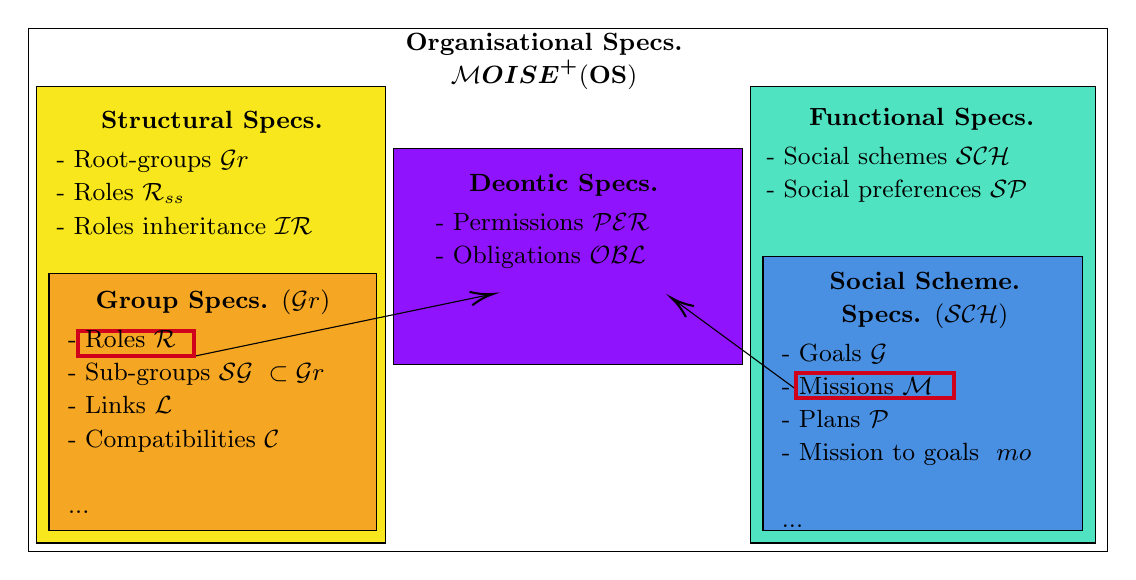
\begin{tikzpicture}[x=0.75pt,y=0.75pt,yscale=-1,xscale=1]
%uncomment if require: \path (0,1656); %set diagram left start at 0, and has height of 1656

%Shape: Rectangle [id:dp6756844921493015] 
\draw  [fill={rgb, 255:red, 248; green, 231; blue, 28 }  ,fill opacity=1 ] (46,1204) -- (214,1204) -- (214,1424) -- (46,1424) -- cycle ;
%Shape: Rectangle [id:dp3759944257810566] 
\draw  [fill={rgb, 255:red, 80; green, 227; blue, 194 }  ,fill opacity=1 ] (390,1204) -- (556,1204) -- (556,1424) -- (390,1424) -- cycle ;
%Shape: Rectangle [id:dp28244406216006945] 
\draw  [fill={rgb, 255:red, 144; green, 19; blue, 254 }  ,fill opacity=1 ] (218,1234) -- (386,1234) -- (386,1338) -- (218,1338) -- cycle ;
%Shape: Rectangle [id:dp32232123359581766] 
\draw   (42,1176) -- (562,1176) -- (562,1428) -- (42,1428) -- cycle ;
%Shape: Rectangle [id:dp7605706269262755] 
\draw  [fill={rgb, 255:red, 74; green, 144; blue, 226 }  ,fill opacity=1 ] (396,1286) -- (550,1286) -- (550,1418) -- (396,1418) -- cycle ;
%Shape: Rectangle [id:dp33110985390647496] 
\draw   (52,1294) -- (210,1294) -- (210,1418) -- (52,1418) -- cycle ;
%Shape: Rectangle [id:dp8653560038381976] 
\draw  [fill={rgb, 255:red, 245; green, 166; blue, 35 }  ,fill opacity=1 ] (52,1294) -- (210,1294) -- (210,1418) -- (52,1418) -- cycle ;
%Straight Lines [id:da09781093164567278] 
\draw    (412,1350) -- (353.61,1307.18) ;
\draw [shift={(352,1306)}, rotate = 36.25] [color={rgb, 255:red, 0; green, 0; blue, 0 }  ][line width=0.75]    (10.93,-3.29) .. controls (6.95,-1.4) and (3.31,-0.3) .. (0,0) .. controls (3.31,0.3) and (6.95,1.4) .. (10.93,3.29)   ;
%Straight Lines [id:da3938396723807833] 
\draw    (122,1334) -- (264.04,1304.41) ;
\draw [shift={(266,1304)}, rotate = 168.23] [color={rgb, 255:red, 0; green, 0; blue, 0 }  ][line width=0.75]    (10.93,-3.29) .. controls (6.95,-1.4) and (3.31,-0.3) .. (0,0) .. controls (3.31,0.3) and (6.95,1.4) .. (10.93,3.29)   ;
%Shape: Rectangle [id:dp269311335478327] 
\draw  [color={rgb, 255:red, 208; green, 2; blue, 27 }  ,draw opacity=1 ][line width=1.5]  (66,1322) -- (122,1322) -- (122,1334) -- (66,1334) -- cycle ;
%Shape: Rectangle [id:dp7449860119164387] 
\draw  [color={rgb, 255:red, 208; green, 2; blue, 27 }  ,draw opacity=1 ][line width=1.5]  (412,1342) -- (488,1342) -- (488,1354) -- (412,1354) -- cycle ;


% Text Node
\draw (472.5,1237.41) node   [align=left] {\begin{minipage}[lt]{112.2pt}\setlength\topsep{0pt}
\begin{center}
\textbf{{\small Functional Specs.}}
\end{center}
{\small  - Social schemes $\displaystyle \mathcal{SCH}$}\\{\small  - Social preferences $\displaystyle \mathcal{SP}$}
\end{minipage}};
% Text Node
\draw (474,1355) node   [align=left] {\begin{minipage}[lt]{103.36pt}\setlength\topsep{0pt}
\begin{center}
\textbf{{\small Social Scheme.}}\\{\small \textbf{Specs. }$\displaystyle (\mathcal{SCH})$}
\end{center}
{\small  - Goals $\displaystyle \mathcal{G}$}\\{\small  - Missions $\displaystyle \mathcal{M}$}\\{\small  - Plans $\displaystyle \mathcal{P}$}\\{\small  - Mission to goals \ $\displaystyle mo$}\\\\{\small  ...}
\end{minipage}};
% Text Node
\draw (131,1356) node   [align=left] {\begin{minipage}[lt]{104.72pt}\setlength\topsep{0pt}
\begin{center}
{\small \textbf{Group Specs. }$\displaystyle (\mathcal{G} r)$}
\end{center}
{\small  - Roles $\displaystyle \mathcal{R}$}\\{\small  - Sub-groups $\displaystyle \mathcal{SG} \ \subset \mathcal{G} r$}\\{\small  - Links $\displaystyle \mathcal{L}$}\\{\small  - Compatibilities $\displaystyle \mathcal{C}$}\\\\{\small  ...}
\end{minipage}};
% Text Node
\draw (181,1177) node [anchor=north west][inner sep=0.75pt]   [align=left] {\begin{minipage}[lt]{162.41pt}\setlength\topsep{0pt}
\begin{center}
{\small \textbf{Organisational Specs. }$\displaystyle \mathcal{M}\boldsymbol{OISE^{+}}$($\displaystyle \mathbf{OS}$)}
\end{center}

\end{minipage}};
% Text Node
\draw (300,1269.09) node   [align=left] {\begin{minipage}[lt]{92.48pt}\setlength\topsep{0pt}
\begin{center}
\textbf{{\small Deontic Specs.}}
\end{center}
{\small  - Permissions $\displaystyle \mathcal{PER}$}\\{\small  - Obligations $\displaystyle \mathcal{OBL}$}
\end{minipage}};
% Text Node
\draw (130.5,1245.69) node   [align=left] {\begin{minipage}[lt]{112.2pt}\setlength\topsep{0pt}
\begin{center}
\textbf{{\small Structural Specs.}}
\end{center}
{\small  - Root-groups $\displaystyle \mathcal{G} r$}\\{\small  - Roles $\displaystyle \mathcal{R}_{ss}$}\\{\small  - Roles inheritance $\displaystyle \mathcal{IR}$}
\end{minipage}};


\end{tikzpicture}
    \caption{\textbf{Une vue synthétique de} $\mathbfcal{M}\mathbf{OISE^+}$}
    \label{fig:moise_model}
\end{figure}

\noindent \textbf{Spécifications structurelles (SS):}
Elles définissent la structure des agents, notées
$
\mathcal{SS} = \langle \mathcal{R}, \mathcal{IR}, \mathcal{G} \rangle,
$
où \(\mathcal{R}\) est l'ensemble des rôles, avec une relation d'héritage \(\mathcal{IR}\) (c'est-à-dire, \(\rho_1 \sqsubset \rho_2\) si \(\rho_1\) hérite de \(\rho_2\)). De plus, \(\mathcal{GR}\) spécifie des groupes sous la forme 
$
\langle \mathcal{R}, \mathcal{SG}, \mathcal{L}^{intra}, \mathcal{L}^{inter}, \mathcal{C}^{intra}, \mathcal{C}^{inter}, np, ng \rangle,
$
où \(\mathcal{L}\) désigne les liens (connaissance, communication, autorité) et \(\mathcal{C}\) les compatibilités entre rôles, avec \(np\) et \(ng\) indiquant respectivement le nombre de rôles et de sous-groupes.

\vspace{0.5em}
\noindent \textbf{Spécifications fonctionnelles (FS):}
Elles décrivent les objectifs des agents et sont notées
$
\mathcal{FS} = \langle \mathcal{SCH}, \mathcal{PO} \rangle.
$
Le schéma social \(\mathcal{SCH}\) comprend les objectifs globaux \(\mathcal{G}\), les missions \(\mathcal{M}\) et les plans \(\mathcal{P}\) organisant ces objectifs (via l'opérateur \(op\) pour séquence, choix ou parallèle). Les missions regroupent des ensembles d'objectifs (\(mo\)) et le nombre d'agents par mission est donné par \(nm\), tandis que \(\mathcal{PO}\) représente les préférences (ex. \(m_1 \prec m_2\)).

\vspace{0.5em}
\noindent \textbf{Spécifications déontiques (DS):}
Elles précisent la relation entre rôles et objectifs, notées
$
\mathcal{DS} = \langle \mathcal{OBL}, \mathcal{PER} \rangle.
$
Les contraintes temporelles \(\mathcal{TC}\) fixent les périodes pour les permissions/obligations (ex. \(Any\) pour tout moment). Les obligations \(\mathcal{OBL}\) imposent aux agents en rôle \(\rho_a\) d'exécuter la mission \(m\) aux moments \(tc\), tandis que les permissions \(\mathcal{PER}\) les autorisent. La fonction \(rds\) associe à chaque rôle une spécification sous la forme 
$
\langle tc, y, m \rangle,
$
avec \(y=0\) pour permission et \(y=1\) pour obligation.


Les autres spécifications structurelles (compatibilités, liens) sont inhérentes aux rôles. De même, les objectifs (incluant missions et \(mo\)) sont inhérents aux autres spécifications fonctionnelles (plans, cardinalités, ordres de préférence). Considérer les rôles, les missions et les permissions/obligations est suffisant pour lier \(\mathcal{M}OISE^+\) au Dec-POMDP.

\begin{figure*}[t]

    \label{eq:single_value_function}
    \raggedright
    \textbf{\textit{Définition 1} \quad Fonction de valeur d'état adaptée aux \textbf{Guide de Contrainte} en mode AEC :}

    \begin{scriptsize}
      \vspace{-0.3cm}
      \begin{gather*}
      V^{\pi^j}(s_t) = \hspace{-0.75cm} \sum_{\textcolor{red}{ \substack{a_{t} \in A \text{ si } rn() < ch_{t}, \\ 
      a_{t} \in A_{t} \text{ sinon}}
      }}{\hspace{-0.7cm} \pi_i(a_{t} | \omega_t)} \sum_{s_{t+1} \in S}{\hspace{-0.1cm} T(s_{t+1} | s_t, a_{t})\Bigl[R(s_t,a_{t},s_{t+1}) + \hspace{-0.1cm} \textcolor{blue}{ \sum_{m \in \mathcal{M}_i}{ \hspace{-0.1cm} v_m(t) \frac{grg_m(h_{t+1})}{1 - p + \epsilon} } } + \textcolor{red}{(1-ch_t) \times rrg(\omega_t,a_{t+1})} + V^{\pi^j_{i+1 \ mod \ n}}(s_{t+1})\Bigr]}
    \end{gather*}  
    %
    \vspace{-0.3cm}
    %
    \textcolor{red}{$\hspace{0cm}\text{Avec } rag(h_t, \omega_t) = A_{t} \times \mathbb{R} \text{, } \langle a_t, ch_{t} \rangle \in A_{t} \times \mathbb{R} \text{ ; et } rn: \emptyset \to [0,1[ \text{, une fonction aléatoire uniforme}$}
    %
    \vspace{-0cm}
    \textcolor{blue}{
    \begin{gather*}
    \hspace{-4.1cm}\text{Avec } \omega_t = O(\omega_t | s_t, a_t) \text{ ; } h_t = \{h_0 = \langle \rangle, h_{t+1} = \langle h_t, \langle \omega_{t+1}, a_{t+1} \rangle \rangle \} \text{ ; } grg_m(h) = \hspace{-0.8cm} \sum_{(grg_i,w_i) \in mo(m)}{\hspace{-0.8cm} w_i \times grg_i(h)} \text{ ; } \epsilon \in \mathbb{R}_{>0} \text{ ; }
    \end{gather*}
    }
    \vspace{-1.05cm}
    \textcolor{blue}{
    \begin{gather*}
    \hspace{-8.5cm}
    v_m(t) = \{ 1 \text{ si } t \in t_c \text{ ; sinon } 0 \} \text{ ; et } \mathcal{M}_i = \{m_j \mid \langle ar(i),m_j,t_c,p \rangle \in \mathcal{M}\}
    \end{gather*}
    }
    \vspace{-0.6cm}

    \end{scriptsize}

\end{figure*}

\subsection{Liaison de \(\mathcal{M}OISE^+\) avec le MARL}

\begin{figure}[h!]

    \adjustbox{lap=-0.38cm}{\tikzset{every picture/.style={line width=0.75pt}} %set default line width to 0.75pt        

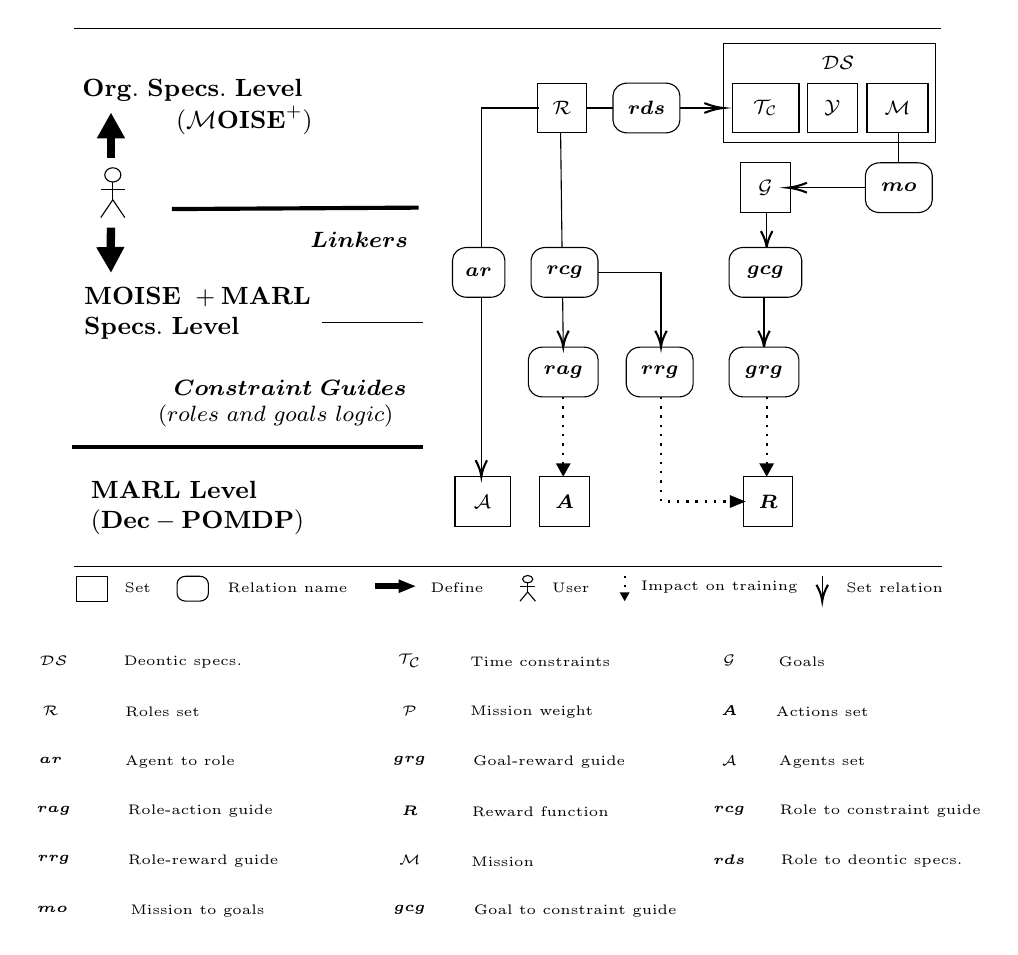
\begin{tikzpicture}[x=0.75pt,y=0.75pt,yscale=-1.2,xscale=1.4]
    %uncomment if require: \path (0,2584); %set diagram left start at 0, and has height of 2584

    %Straight Lines [id:da4973066741986565] 
    \draw [line width=1.5]    (118.21,2302.58) -- (203.1,2302) ;
    %Straight Lines [id:da14807114776731778] 
    \draw    (368.35,2272) -- (368.35,2294) -- (332.16,2294) ;
    \draw [shift={(330.16,2294)}, rotate = 360] [color={rgb, 255:red, 0; green, 0; blue, 0 }  ][line width=0.75]    (6.56,-1.97) .. controls (4.17,-0.84) and (1.99,-0.18) .. (0,0) .. controls (1.99,0.18) and (4.17,0.84) .. (6.56,1.97)   ;
    %Straight Lines [id:da16285043353898754] 
    \draw [line width=1.5]    (83.88,2398) -- (204.61,2398) ;
    %Straight Lines [id:da6299512000169913] 
    \draw    (169.94,2348) -- (204.61,2348) ;
    %Straight Lines [id:da64750232417664] 
    \draw    (84.65,2446) -- (383.15,2446) ;
    %Straight Lines [id:da35895220906699743] 
    \draw    (84.65,2230) -- (383,2230) ;
    %Straight Lines [id:da715014372569708] 
    \draw    (244.68,2262) -- (224.68,2262) -- (224.68,2408) ;
    \draw [shift={(224.68,2410)}, rotate = 270] [color={rgb, 255:red, 0; green, 0; blue, 0 }  ][line width=0.75]    (6.56,-1.97) .. controls (4.17,-0.84) and (1.99,-0.18) .. (0,0) .. controls (1.99,0.18) and (4.17,0.84) .. (6.56,1.97)   ;
    %Straight Lines [id:da71870438525014] 
    \draw    (251.96,2328) -- (286.51,2328) -- (286.51,2356) ;
    \draw [shift={(286.51,2358)}, rotate = 270] [color={rgb, 255:red, 0; green, 0; blue, 0 }  ][line width=0.75]    (6.56,-1.97) .. controls (4.17,-0.84) and (1.99,-0.18) .. (0,0) .. controls (1.99,0.18) and (4.17,0.84) .. (6.56,1.97)   ;
    %Straight Lines [id:da6006267784187092] 
    \draw [line width=0.75]  [dash pattern={on 0.84pt off 2.51pt}]  (252.87,2378) -- (252.87,2407) ;
    \draw [shift={(252.87,2410)}, rotate = 270] [fill={rgb, 255:red, 0; green, 0; blue, 0 }  ][line width=0.08]  [draw opacity=0] (5.36,-2.57) -- (0,0) -- (5.36,2.57) -- cycle    ;
    %Straight Lines [id:da8743336135156266] 
    \draw    (322.88,2304) -- (322.88,2316) ;
    \draw [shift={(322.88,2318)}, rotate = 270] [color={rgb, 255:red, 0; green, 0; blue, 0 }  ][line width=0.75]    (6.56,-1.97) .. controls (4.17,-0.84) and (1.99,-0.18) .. (0,0) .. controls (1.99,0.18) and (4.17,0.84) .. (6.56,1.97)   ;
    %Straight Lines [id:da14641229967966152] 
    \draw [line width=0.75]  [dash pattern={on 0.84pt off 2.51pt}]  (322.88,2378) -- (322.88,2407) ;
    \draw [shift={(322.88,2410)}, rotate = 270] [fill={rgb, 255:red, 0; green, 0; blue, 0 }  ][line width=0.08]  [draw opacity=0] (5.36,-2.57) -- (0,0) -- (5.36,2.57) -- cycle    ;
    %Straight Lines [id:da9260929933425808] 
    \draw [line width=0.75]  [dash pattern={on 0.84pt off 2.51pt}]  (286.51,2378) -- (286.51,2420) -- (312.61,2420) ;
    \draw [shift={(315.61,2420)}, rotate = 180] [fill={rgb, 255:red, 0; green, 0; blue, 0 }  ][line width=0.08]  [draw opacity=0] (5.36,-2.57) -- (0,0) -- (5.36,2.57) -- cycle    ;
    %Straight Lines [id:da3057006030233673] 
    \draw [line width=0.75]  [dash pattern={on 0.84pt off 2.51pt}]  (274,2449.7) -- (274,2457) ;
    \draw [shift={(274,2460)}, rotate = 270] [fill={rgb, 255:red, 0; green, 0; blue, 0 }  ][line width=0.08]  [draw opacity=0] (3.57,-1.72) -- (0,0) -- (3.57,1.72) -- cycle    ;
    %Straight Lines [id:da07288166228322246] 
    \draw    (342,2449.98) -- (342,2458) ;
    \draw [shift={(342,2460)}, rotate = 270] [color={rgb, 255:red, 0; green, 0; blue, 0 }  ][line width=0.75]    (6.56,-1.97) .. controls (4.17,-0.84) and (1.99,-0.18) .. (0,0) .. controls (1.99,0.18) and (4.17,0.84) .. (6.56,1.97)   ;
    %Shape: Ellipse [id:dp8508274348425935] 
    \draw   (95.09,2288.86) .. controls (95.09,2287.28) and (96.33,2286) .. (97.85,2286) .. controls (99.38,2286) and (100.62,2287.28) .. (100.62,2288.86) .. controls (100.62,2290.44) and (99.38,2291.71) .. (97.85,2291.71) .. controls (96.33,2291.71) and (95.09,2290.44) .. (95.09,2288.86) -- cycle ;
    %Straight Lines [id:da3825450168053828] 
    \draw    (97.85,2291.71) -- (97.85,2298.86) ;
    %Straight Lines [id:da521321206042058] 
    \draw    (97.85,2298.86) -- (93.71,2306) ;
    %Straight Lines [id:da055514206493922025] 
    \draw    (97.85,2298.86) -- (102,2306) ;
    %Straight Lines [id:da8996496708356774] 
    \draw    (102,2294.57) -- (93.71,2294.57) ;

    %Straight Lines [id:da31678488015771755] 
    \draw [line width=2.25]    (188,2454) -- (196.97,2454) ;
    \draw [shift={(201.97,2454)}, rotate = 180] [fill={rgb, 255:red, 0; green, 0; blue, 0 }  ][line width=0.08]  [draw opacity=0] (5.72,-2.75) -- (0,0) -- (5.72,2.75) -- cycle    ;
    %Shape: Ellipse [id:dp3927356466672782] 
    \draw   (238.88,2451.17) .. controls (238.88,2450.36) and (239.67,2449.7) .. (240.64,2449.7) .. controls (241.61,2449.7) and (242.4,2450.36) .. (242.4,2451.17) .. controls (242.4,2451.99) and (241.61,2452.65) .. (240.64,2452.65) .. controls (239.67,2452.65) and (238.88,2451.99) .. (238.88,2451.17) -- cycle ;
    %Straight Lines [id:da3365602555559104] 
    \draw    (240.64,2452.65) -- (240.64,2456.32) ;
    %Straight Lines [id:da7990875235744026] 
    \draw    (240.64,2456.32) -- (238,2460) ;
    %Straight Lines [id:da23945649338821617] 
    \draw    (240.64,2456.32) -- (243.28,2460) ;
    %Straight Lines [id:da11927353559661591] 
    \draw    (243.28,2454.12) -- (238,2454.12) ;

    %Straight Lines [id:da5816423191130675] 
    \draw    (251.96,2272) -- (252.85,2356) ;
    \draw [shift={(252.87,2358)}, rotate = 269.39] [color={rgb, 255:red, 0; green, 0; blue, 0 }  ][line width=0.75]    (6.56,-1.97) .. controls (4.17,-0.84) and (1.99,-0.18) .. (0,0) .. controls (1.99,0.18) and (4.17,0.84) .. (6.56,1.97)   ;
    %Straight Lines [id:da9310455126832857] 
    \draw    (321.97,2338) -- (321.97,2356) ;
    \draw [shift={(321.97,2358)}, rotate = 270] [color={rgb, 255:red, 0; green, 0; blue, 0 }  ][line width=0.75]    (6.56,-1.97) .. controls (4.17,-0.84) and (1.99,-0.18) .. (0,0) .. controls (1.99,0.18) and (4.17,0.84) .. (6.56,1.97)   ;
    %Shape: Rectangle [id:dp293492578719597] 
    \draw   (120,2453) .. controls (120,2451.34) and (121.34,2450) .. (123,2450) -- (127.72,2450) .. controls (129.37,2450) and (130.72,2451.34) .. (130.72,2453) -- (130.72,2457) .. controls (130.72,2458.66) and (129.37,2460) .. (127.72,2460) -- (123,2460) .. controls (121.34,2460) and (120,2458.66) .. (120,2457) -- cycle ;
    %Straight Lines [id:da33566712615128225] 
    \draw    (261.05,2262) -- (306,2262) ;
    \draw [shift={(308,2262)}, rotate = 180] [color={rgb, 255:red, 0; green, 0; blue, 0 }  ][line width=0.75]    (6.56,-1.97) .. controls (4.17,-0.84) and (1.99,-0.18) .. (0,0) .. controls (1.99,0.18) and (4.17,0.84) .. (6.56,1.97)   ;
    %Shape: Rectangle [id:dp28383270948937667] 
    \draw   (308,2236) -- (381.08,2236) -- (381.08,2276) -- (308,2276) -- cycle ;
    %Straight Lines [id:da18020989903965012] 
    \draw [line width=3]    (97.22,2282) -- (97.22,2270) ;
    \draw [shift={(97.22,2264)}, rotate = 90] [fill={rgb, 255:red, 0; green, 0; blue, 0 }  ][line width=0.08]  [draw opacity=0] (10.18,-4.89) -- (0,0) -- (10.18,4.89) -- cycle    ;
    %Straight Lines [id:da018421338049046554] 
    \draw [line width=3]    (97.22,2310) -- (97.11,2322.37) ;
    \draw [shift={(97.22,2328)}, rotate = 268.86] [fill={rgb, 255:red, 0; green, 0; blue, 0 }  ][line width=0.08]  [draw opacity=0] (10.18,-4.89) -- (0,0) -- (10.18,4.89) -- cycle    ;
    %Shape: Rectangle [id:dp7281037051878541] 
    \draw   (85.42,2450) -- (96.13,2450) -- (96.13,2460) -- (85.42,2460) -- cycle ;

    % Text Node
    \draw (362,2544.5) node  [font=\tiny] [align=left] {Role to constraint guide};
    % Text Node
    \draw (342,2524.5) node  [font=\tiny] [align=left] {Agents set};
    % Text Node
    \draw (342,2504.5) node  [font=\tiny] [align=left] {Actions set};
    % Text Node
    \draw (257,2584.5) node  [font=\tiny] [align=left] {Goal to constraint guide};
    % Text Node
    \draw (335,2484.5) node  [font=\tiny] [align=left] {Goals};
    % Text Node
    \draw (359,2564.5) node  [font=\tiny] [align=left] {Role to deontic specs.};
    % Text Node
    \draw (232,2564.5) node  [font=\tiny] [align=left] {Mission};
    % Text Node
    \draw (245,2544.5) node  [font=\tiny] [align=left] {Reward function};
    % Text Node
    \draw (248,2524.5) node  [font=\tiny] [align=left] {Goal-reward guide};
    % Text Node
    \draw (242,2504.5) node  [font=\tiny] [align=left] {Mission weight};
    % Text Node
    \draw (245,2484.5) node  [font=\tiny] [align=left] {Time constraints};
    % Text Node
    \draw (127,2584.5) node  [font=\tiny] [align=left] {Mission to goals};
    % Text Node
    \draw (129,2564.5) node  [font=\tiny] [align=left] {Role-reward guide};
    % Text Node
    \draw (128,2544.5) node  [font=\tiny] [align=left] {Role-action guide};
    % Text Node
    \draw (121,2524.5) node  [font=\tiny] [align=left] {Agent to role};
    % Text Node
    \draw (115,2504.5) node  [font=\tiny] [align=left] {Roles set};
    % Text Node
    \draw (122,2484.5) node  [font=\tiny] [align=left] {Deontic specs.};
    % Text Node
    \draw (310,2544) node  [font=\tiny] [align=left] {$\displaystyle \boldsymbol{rcg}$};
    % Text Node
    \draw (200,2504) node  [font=\tiny] [align=left] {$\displaystyle \mathcal{P}$};
    % Text Node
    \draw (200,2484) node  [font=\tiny] [align=left] {$\displaystyle \mathcal{T_{C}}$};
    % Text Node
    \draw (200,2564) node  [font=\tiny] [align=left] {$\displaystyle \mathcal{M}$};
    % Text Node
    \draw (77.5,2484) node  [font=\tiny] [align=left] {$\displaystyle \mathcal{DS}$};
    % Text Node
    \draw (310,2564) node  [font=\tiny] [align=left] {$\displaystyle \boldsymbol{rds}$};
    % Text Node
    \draw (310,2504) node  [font=\tiny] [align=left] {$\displaystyle \boldsymbol{A}$};
    % Text Node
    \draw (200,2544) node  [font=\tiny] [align=left] {$\displaystyle \boldsymbol{R}$};
    % Text Node
    \draw (310,2524) node  [font=\tiny] [align=left] {$\displaystyle \mathcal{A}$};
    % Text Node
    \draw (200,2524) node  [font=\tiny] [align=left] {$\displaystyle \boldsymbol{grg}$};
    % Text Node
    \draw (77.5,2564) node  [font=\tiny] [align=left] {$\displaystyle \boldsymbol{rrg}$};
    % Text Node
    \draw (77.5,2544) node  [font=\tiny] [align=left] {$\displaystyle \boldsymbol{rag}$};
    % Text Node
    \draw (200,2584) node  [font=\tiny] [align=left] {$\displaystyle \boldsymbol{gcg}$};
    % Text Node
    \draw (76.5,2524) node  [font=\tiny] [align=left] {$\displaystyle \boldsymbol{ar}$};
    % Text Node
    \draw (77,2584) node  [font=\tiny] [align=left] {$\displaystyle \boldsymbol{mo}$};
    % Text Node
    \draw (76.5,2504) node  [font=\tiny] [align=left] {$\displaystyle \mathcal{R}$};
    % Text Node
    \draw (310,2484) node  [font=\tiny] [align=left] {$\displaystyle \mathcal{G}$};


    % Text Node
    \draw  [fill={rgb, 255:red, 255; green, 255; blue, 255 }  ,fill opacity=1 ]  (241.82,2323) .. controls (241.82,2320.24) and (244.06,2318) .. (246.82,2318) -- (259.82,2318) .. controls (262.58,2318) and (264.82,2320.24) .. (264.82,2323) -- (264.82,2333) .. controls (264.82,2335.76) and (262.58,2338) .. (259.82,2338) -- (246.82,2338) .. controls (244.06,2338) and (241.82,2335.76) .. (241.82,2333) -- cycle  ;
    \draw (253.32,2328) node  [font=\scriptsize] [align=left] {$\displaystyle \boldsymbol{rcg}$};
    % Text Node
    \draw    (337,2252) -- (354,2252) -- (354,2272) -- (337,2272) -- cycle  ;
    \draw (345.5,2262) node  [font=\scriptsize] [align=left] {$\displaystyle \mathcal{Y}$};
    % Text Node
    \draw    (311,2252) -- (334,2252) -- (334,2272) -- (311,2272) -- cycle  ;
    \draw (322.5,2262) node  [font=\scriptsize] [align=left] {$\displaystyle \mathcal{T_{C}}$};
    % Text Node
    \draw    (357.39,2252) -- (378.39,2252) -- (378.39,2272) -- (357.39,2272) -- cycle  ;
    \draw (367.89,2262) node  [font=\scriptsize] [align=left] {$\displaystyle \mathcal{M}$};
    % Text Node
    \draw (347.43,2244) node  [font=\scriptsize] [align=left] {$\displaystyle \mathcal{DS}$};
    % Text Node
    \draw  [fill={rgb, 255:red, 255; green, 255; blue, 255 }  ,fill opacity=1 ]  (270,2257) .. controls (270,2254.24) and (272.24,2252) .. (275,2252) -- (288,2252) .. controls (290.76,2252) and (293,2254.24) .. (293,2257) -- (293,2267) .. controls (293,2269.76) and (290.76,2272) .. (288,2272) -- (275,2272) .. controls (272.24,2272) and (270,2269.76) .. (270,2267) -- cycle  ;
    \draw (281.5,2262) node  [font=\scriptsize] [align=left] {$\displaystyle \boldsymbol{rds}$};
    % Text Node
    \draw (158,2454.5) node  [font=\tiny] [align=left] {Relation name};
    % Text Node
    \draw (106.46,2454.5) node  [font=\tiny] [align=left] {Set};
    % Text Node
    \draw (255.47,2454.5) node  [font=\tiny] [align=left] {User};
    % Text Node
    \draw (216.32,2454.5) node  [font=\tiny] [align=left] {Define};
    % Text Node
    \draw (366.91,2454.5) node  [font=\tiny] [align=left] {Set relation};
    % Text Node
    \draw (306.61,2454.5) node  [font=\tiny] [align=left] {Impact on training};
    % Text Node
    \draw    (244.82,2410) -- (261.82,2410) -- (261.82,2430) -- (244.82,2430) -- cycle  ;
    \draw (253.32,2420) node  [font=\scriptsize] [align=left] {$\displaystyle \boldsymbol{A}$};
    % Text Node
    \draw    (314.84,2410) -- (331.84,2410) -- (331.84,2430) -- (314.84,2430) -- cycle  ;
    \draw (323.34,2420) node  [font=\scriptsize] [align=left] {$\displaystyle \boldsymbol{R}$};
    % Text Node
    \draw    (215.63,2410) -- (234.63,2410) -- (234.63,2430) -- (215.63,2430) -- cycle  ;
    \draw (225.13,2420) node  [font=\scriptsize] [align=left] {$\displaystyle \mathcal{A}$};
    % Text Node
    \draw  [fill={rgb, 255:red, 255; green, 255; blue, 255 }  ,fill opacity=1 ]  (309.97,2363) .. controls (309.97,2360.24) and (312.21,2358) .. (314.97,2358) -- (328.97,2358) .. controls (331.73,2358) and (333.97,2360.24) .. (333.97,2363) -- (333.97,2373) .. controls (333.97,2375.76) and (331.73,2378) .. (328.97,2378) -- (314.97,2378) .. controls (312.21,2378) and (309.97,2375.76) .. (309.97,2373) -- cycle  ;
    \draw (321.97,2368) node  [font=\scriptsize] [align=left] {$\displaystyle \boldsymbol{grg}$};
    % Text Node
    \draw    (274.56,2363) .. controls (274.56,2360.24) and (276.8,2358) .. (279.56,2358) -- (292.56,2358) .. controls (295.32,2358) and (297.56,2360.24) .. (297.56,2363) -- (297.56,2373) .. controls (297.56,2375.76) and (295.32,2378) .. (292.56,2378) -- (279.56,2378) .. controls (276.8,2378) and (274.56,2375.76) .. (274.56,2373) -- cycle  ;
    \draw (286.06,2368) node  [font=\scriptsize] [align=left] {$\displaystyle \boldsymbol{rrg}$};
    % Text Node
    \draw    (240.87,2363) .. controls (240.87,2360.24) and (243.11,2358) .. (245.87,2358) -- (259.87,2358) .. controls (262.63,2358) and (264.87,2360.24) .. (264.87,2363) -- (264.87,2373) .. controls (264.87,2375.76) and (262.63,2378) .. (259.87,2378) -- (245.87,2378) .. controls (243.11,2378) and (240.87,2375.76) .. (240.87,2373) -- cycle  ;
    \draw (252.87,2368) node  [font=\scriptsize] [align=left] {$\displaystyle \boldsymbol{rag}$};
    % Text Node
    \draw (156.15,2380.5) node  [font=\footnotesize] [align=left] {$\displaystyle  \begin{array}{{>{\displaystyle}l}}
                \ \ \boldsymbol{Constraint\ Guides} \\
                ( roles\ and\ goals\ logic)
            \end{array}$};
    % Text Node
    \draw  [fill={rgb, 255:red, 255; green, 255; blue, 255 }  ,fill opacity=1 ]  (309.93,2323) .. controls (309.93,2320.24) and (312.17,2318) .. (314.93,2318) -- (329.93,2318) .. controls (332.69,2318) and (334.93,2320.24) .. (334.93,2323) -- (334.93,2333) .. controls (334.93,2335.76) and (332.69,2338) .. (329.93,2338) -- (314.93,2338) .. controls (312.17,2338) and (309.93,2335.76) .. (309.93,2333) -- cycle  ;
    \draw (322.43,2328) node  [font=\scriptsize] [align=left] {$\displaystyle \boldsymbol{gcg}$};
    % Text Node
    \draw  [fill={rgb, 255:red, 255; green, 255; blue, 255 }  ,fill opacity=1 ]  (214.77,2323) .. controls (214.77,2320.24) and (217.01,2318) .. (219.77,2318) -- (227.77,2318) .. controls (230.53,2318) and (232.77,2320.24) .. (232.77,2323) -- (232.77,2333) .. controls (232.77,2335.76) and (230.53,2338) .. (227.77,2338) -- (219.77,2338) .. controls (217.01,2338) and (214.77,2335.76) .. (214.77,2333) -- cycle  ;
    \draw (223.77,2328) node  [font=\scriptsize] [align=left] {$\displaystyle \boldsymbol{ar}$};
    % Text Node
    \draw  [fill={rgb, 255:red, 255; green, 255; blue, 255 }  ,fill opacity=1 ]  (356.85,2289) .. controls (356.85,2286.24) and (359.08,2284) .. (361.85,2284) -- (374.85,2284) .. controls (377.61,2284) and (379.85,2286.24) .. (379.85,2289) -- (379.85,2299) .. controls (379.85,2301.76) and (377.61,2304) .. (374.85,2304) -- (361.85,2304) .. controls (359.08,2304) and (356.85,2301.76) .. (356.85,2299) -- cycle  ;
    \draw (368.35,2294) node  [font=\scriptsize] [align=left] {$\displaystyle \boldsymbol{mo}$};
    % Text Node
    \draw (127,2344.5) node  [font=\small] [align=left] {$\displaystyle  \begin{array}{{>{\displaystyle}l}}
                \mathbf{MOISE\ +MARL} \\
                \mathbf{Specs.\ Level}
            \end{array}$};
    % Text Node
    \draw (127,2422.5) node  [font=\small] [align=left] {$\displaystyle  \begin{array}{{>{\displaystyle}l}}
                \mathbf{MARL\ Level} \\
                \mathbf{(Dec-POMDP)}
            \end{array}$};
    % Text Node
    \draw    (243.91,2252) -- (260.91,2252) -- (260.91,2272) -- (243.91,2272) -- cycle  ;
    \draw (252.41,2262) node  [font=\scriptsize] [align=left] {$\displaystyle \mathcal{R}$};
    % Text Node
    \draw (182.64,2315) node  [font=\footnotesize] [align=left] {$\displaystyle \boldsymbol{Linkers}$};
    % Text Node
    \draw    (313.93,2284) -- (330.93,2284) -- (330.93,2304) -- (313.93,2304) -- cycle  ;
    \draw (322.43,2294) node  [font=\scriptsize] [align=left] {$\displaystyle \mathcal{G}$};
    % Text Node
    \draw (127,2261.5) node  [font=\small] [align=left] {$\displaystyle  \begin{array}{{>{\displaystyle}l}}
                \mathbf{{\displaystyle Org.\ Specs.\ Level}} \\
                {\displaystyle \ \ \ \ \ \ \ \ \ \ \ (\mathcal{M}\mathbf{OISE^+})}
            \end{array}$};


\end{tikzpicture}}
    \caption{\textbf{Une vue minimale du cadre MOISE+MARL} :
    Les utilisateurs définissent d'abord les spécifications de \(\mathcal{M}OISE^+\), qui incluent des rôles (\(\mathcal{R}\)) et des missions (\(\mathcal{M}\)) associées via \(rds\). Ensuite, ils créent des spécifications MOISE+MARL en définissant d'abord des \textbf{Guide de Contraintes} tels que \(rag\) et \(rrg\) pour spécifier la logique des rôles, et \(grg\) pour la logique des objectifs.
    Ensuite, des \textbf{Lieurs} sont utilisés pour connecter les agents aux rôles via \(ar\) et pour relier la logique des \textbf{Guide de Contrainte} aux spécifications définies de \(\mathcal{M}OISE^+\). Une fois cette configuration réalisée, des rôles peuvent être attribués aux agents, et le cadre MARL s'adapte en conséquence pendant l'entraînement.
    }
    \label{fig:mm_synthesis}
\end{figure}

Alors qu'\textit{AGR}~\cite{ferber2003} (Agent Group Role) est un cadre informel qui introduit des rôles par groupes, \(\mathcal{M}OISE^+\) offre une description plus détaillée et flexible des structures et fonctions d'un système multi-agent (MAS), facilitant ainsi la formalisation des politiques en MARL.

\medskip
\noindent \textbf{Guides de Contraintes} : Trois relations décrivent la logique des rôles et objectifs dans le cadre Dec-POMDP :
i) \textbf{Guide d'action de rôle} \(rag: H \times \Omega \to \mathcal{P}(A \times \mathbb{R})\) : Pour chaque couple \((h,\omega)\) (\(h\in H\), \(\omega\in \Omega\)), il associe un ensemble d'actions \(A_\omega \subseteq A\) avec une rigidité \(ch \in [0,1]\) (par défaut \(ch=1\)), restreignant ainsi le choix de la prochaine action ; \quad
ii) \textbf{Guide de récompense de rôle} \(rrg: H \times \Omega \times A \to \mathbb{R}\) : Défini par \(rrg(h,\omega,a)=r_m\) si \(a \notin A_\omega\) (avec \(rag(h,\omega)=A_\omega \times \mathbb{R}\)), et 0 sinon, afin d'encourager le respect du rôle ; \quad
iii) \textbf{Guide de récompense d'objectif} \(grg: H \to \mathbb{R}\) : Attribue un bonus \(r_b\) à la récompense globale si \(h\) contient une sous-séquence caractéristique \(h_g \in H_g\) correspondant à un objectif.

\medskip
\noindent \textbf{Lieurs} : Relient les spécifications de \(\mathcal{M}OISE^+\) aux Guides de Contraintes et aux agents :
i) \textbf{Agent vers Rôle} \(ar: \mathcal{A} \to \mathcal{R}\) (relation bijective) ; \quad
ii) \textbf{Rôle vers Guide de Contrainte} \(rcg: \mathcal{R} \to rag \cup rrg\) : Associe à chaque rôle une relation \(rag\) ou \(rrg\) ; \quad
iii) \textbf{Objectif vers Guide de Contrainte} \(gcg: \mathcal{G} \to grg\) : Relie chaque objectif à son guide \(grg\).

\textbf{La résolution du problème MOISE+MARL} consiste à trouver une politique conjointe 
$
\pi^j = \{\pi^j_0, \pi^j_1, \dots, \pi^j_n\}
$
maximisant la fonction de valeur d'état \(V^{\pi^j}\) (ou atteignant un seuil minimal), qui représente la récompense cumulative attendue à partir d'un état initial \(s \in S\) en suivant les actions conjointes \(a^j \in A^n\) sous l'effet de \textbf{Guides de Contraintes}. Cette fonction est définie pour des agents agissant de manière séquentielle et cyclique (mode AEC) (voir la \hyperref[eq:single_value_function]{Définition 1}). La \autoref{fig:mm_synthesis} illustre les liens entre \(\mathcal{M}OISE^+\) et le Dec-POMDP via MOISE+MARL.

À chaque instant \(t \in \mathbb{N}\) (initialement \(t=0\)), l'agent \(i = t \mod n\) doit assumer le rôle \(\rho_i = ar(i)\). Pour chaque spécification déontique valide 
$
d_i = rds(\rho_i) = \langle tc_i, y_i, m_i \rangle,
$
l'agent est autorisé (si \(y_i=0\)) ou obligé (si \(y_i=1\)) d'exécuter la mission \(m_i \in \mathcal{M}\) (avec \(\mathcal{G}_{m_i} = mo(m_i)\)). L'agent choisit d'abord une action parmi celles attendues \(A_t\) si une valeur aléatoire est inférieure à la rigidité \(ch_t\), sinon parmi l'ensemble \(A\); ainsi, un \(ch_t = 1\) impose une contrainte forte.

L'action appliquée à \(s_t\) conduit à l'état suivant \(s_{t+1}\), génère la prochaine observation \(\omega_{t+1}\) et une récompense. Celle-ci est la somme de la récompense globale et des ajustements organisationnels : 
i) un bonus (via les Guides de Récompense d'Objectif), pondéré par \(\frac{1}{1-p+\epsilon}\) pour ajuster son impact, et
ii) une pénalité (via les Guides de Récompense de Rôle), pondérée par la rigidité \(ch_t\) pour ajuster son impact.
Le calcul de la récompense cumulative se poursuit dans \(s_{t+1}\) avec l'agent suivant \((i+1) \mod n\).

\subsection{Faciliter l'implémentation des \textbf{Guide de Contrainte}}

Puisque les rôles, objectifs et missions sont de simples étiquettes, leur définition est implicite. Cependant, implémenter une relation \(rag\), \(rrg\) ou \(grg\) nécessite de définir de nombreux historiques, souvent redondants, rendant une définition extensionnelle fastidieuse. De plus, la logique de chaque \textbf{Guide de Contrainte} analyse la trajectoire de l'agent pour vérifier son appartenance à un ensemble prédéfini. Par exemple, \(rag\) détermine les actions attendues selon l'appartenance de la trajectoire à un ensemble donné et la nouvelle observation.

Une approche consiste à laisser l'utilisateur définir ses \textbf{Guides de Contrainte} via une logique personnalisée (par script, par exemple). Dans ce cas, la relation \(b_g: H \to \{0,1\}\) formalise la décision d'appartenance d'un historique à un ensemble \(H_g\).
Pour simplifier l'implémentation, nous proposons un \textit{Trajectory-based Pattern} (TP), inspiré du Traitement Automatique du Langage, noté \(p \in P\), permettant de définir intentionnellement un ensemble d'historiques.

Un TP implique que toute observation ou action réelle considérée est connue et associée à une étiquette \(l \in L\) (via \(l: \Omega \cup A \to L\)) afin d'être gérée de manière pratique. Un TP \(p \in P\) est défini comme suit : \(p\) est soit une « séquence feuille » notée comme un couple historique-cardinalité \(s_l = \langle h, \{c_{min}, c_{max}\} \rangle\) (où \(h \in H\), \(c_{min} \in \mathbb{N}\), \(c_{max} \in \mathbb{N} \cup \{``*"\}\)) ; soit une « séquence nœud » notée comme un couple composé d'un tuple de séquences et d'une cardinalité \(s_n = \langle \langle s_{l_1}, s_{l_2}, \dots \rangle, \{c_{min}, c_{max}\} \rangle\). Par exemple, le pattern 
$
p = ``[o_1,a_1,[o_2,a_2]\langle0,2\rangle]\langle1,*\rangle"
$
peut être formalisé comme la séquence nœud
$
\langle \langle \langle o_1,a_1\rangle,\langle 1,1 \rangle \rangle, \langle \langle o_2,a_2\rangle,\langle 0,2 \rangle \rangle \rangle \langle 1,``*"\rangle,
$
indiquant l'ensemble des historiques \(H_p\) contenant au moins une fois la sous-séquence constituée d'une première paire \(\langle o_1,a_1\rangle\) suivie d'au maximum deux répétitions de la paire \(\langle o_2,a_2\rangle\).

% La relation \(b_g\) devient alors 
% $
% b_g(h) = m(p_g,h), \quad \text{avec } m: P \times H \to \{0,1\},
% $
% indiquant si un historique \(h \in H\) correspond à un pattern d'historique \(p \in P\) décrivant un ensemble d'historiques \(H_g\).

\section{La méthode TEMM}
\label{sec:TEMM_algorithm}

Comme indiqué en \autoref{sec:related_works}, aucune méthode existante ne répond pleinement à nos exigences pour déterminer les rôles et objectifs implicites ainsi que l'adéquation organisationnelle. Nous proposons donc la méthode \textit{Trajectory-based Evaluation in MOISE+MARL} (TEMM) pour inférer et évaluer des rôles et des missions.

TEMM repose sur l'apprentissage non supervisé pour généraliser ces spécifications à partir des trajectoires collectées lors de multiples épisodes. En quantifiant l'écart entre les spécifications implicites inférées et les comportements observés, TEMM mesure l'adéquation organisationnelle, c'est-à-dire la conformité d'une politique aux spécifications inférées. TEMM repose sur des définitions propres à chaque spécification organisationnelle de \(\mathcal{M}OISE^+\) (historiques conjoints, etc.), inférées progressivement via des techniques non supervisées. Une description informelle est disponible~\hyperref[fn:github]{\footnotemark[1]}.

\footnotetext[1]{Plus de détails, le code et les ensembles de données (hyperparamètres et spécifications) sont disponibles sur \url{https://github.com/julien6/MOISE-MARL}.}

\noindent\textbf{1) Inférence des rôles et héritage} \\
Un rôle \(\rho\) est défini comme une politique dont l'historique contient une Séquence Commune la Plus Longue (SCL). Un rôle \(\rho_2\) hérite de \(\rho_1\) si sa SCL est incluse dans celle de \(\rho_1\). TEMM emploie le clustering hiérarchique pour extraire ces SCL, représentées sous forme de dendrogramme, et mesure l'écart entre les séquences actuelles et inférées, définissant ainsi l'adéquation organisationnelle structurelle.

\noindent\textbf{2) Inférence des objectifs, plans et missions} \\
Un objectif correspond à un ensemble d'observations conjointes communes, atteint via les historiques d'agents performants. TEMM construit pour chaque historique conjoint un graphe de transition, fusionne ces graphes et, à l'aide de K-means, identifie des groupes de trajectoires. Les ensembles d'observations restreints extraits pour chaque groupe sont considérés comme des objectifs implicites, permettant d'inférer les plans sur la base des choix et séquences. Une mission est définie comme l'ensemble des objectifs réalisés par un ou plusieurs agents, et la distance entre les objectifs inférés et l'observation conjointe actuelle permet de calculer l'adéquation organisationnelle structurelle.

\noindent\textbf{3) Inférence des obligations et permissions} \\
Une obligation se produit lorsqu'un agent, jouant le rôle \(\rho\), réalise exclusivement les objectifs d'une mission dans un intervalle donné, tandis qu'une permission permet d'atteindre d'autres objectifs sous conditions. TEMM identifie l'association agent-mission et détermine si l'agent est contraint (obligation) ou bénéficie de flexibilité (permission). L'adéquation organisationnelle globale est la somme de l'adéquation structurelle et fonctionnelle.

Globalement, bien que le K-means et le clustering hiérarchique requièrent une configuration manuelle pour éviter les erreurs, TEMM recommande de vérifier et d'ajuster manuellement les rôles et objectifs obtenus pour éliminer les perturbations éventuelles.


\section{Cadre expérimental}
\label{sec:experimental_setup}

Cette section détaille le cadre expérimental utilisé pour évaluer le cadre MOISE+MARL.

\subsection{Implémentation de MOISE+MARL}

Nous avons développé une API Python, \textquote{MMA}~\hyperref[fn:github]{\footnotemark[1]}, pour implémenter MOISE+MARL. Cette API structure le modèle \(\mathcal{M}OISE^+\) en classes de données imbriquées (la classe « Moise » étant à la racine) afin de définir les spécifications organisationnelles (rôles, objectifs, permissions).

Nus utilisons la bibliothèque \textit{PettingZoo}~\cite{terry2020pettingzoo} (similaire à Gymnasium~\cite{kwiatkowski2024}) pour la gestion des environnements en y intégrant un dictionnaire personnalisable pour le mappage des étiquettes d'observation/action (\(l\)), ainsi que le support des TPs pour définir et faire correspondre les motifs.

Chaque \textbf{Guide de Contrainte} (\(rag\), \(rrg\) et \(grg\)) est implémenté comme une classe distincte. Les utilisateurs peuvent les définir via des fonctions personnalisées ou des règles JSON (par exemple, \(rag\) associe un couple \(\langle\)TP, dernière observation\(\rangle\) à des actions attendues, et \(grg\) applique des bonus selon des TP spécifiques). La classe globale MMA intègre ces guides et relie les agents aux rôles via des relations telles que \(ar\), intégrant ainsi les spécifications de \(\mathcal{M}OISE^+\).

Une fois configuré, MMA encapsule l'environnement avec un wrapper \textit{PettingZoo} qui applique des masques d'actions et ajuste les récompenses pour garantir le respect des spécifications durant l'entraînement. Il intègre également \textit{MARLlib}~\cite{hu2021marlib} pour accéder aux algorithmes MARL de pointe sur un cluster haute performance.

Enfin, la méthode TEMM, avec des hyperparamètres optimisés manuellement, est utilisée après l'entraînement pour inférer les rôles et objectifs implicites via clustering hiérarchique et K-means. Cette analyse génère des sorties visuelles (dendrogrammes, graphes de transition) et permet d'exporter les trajectoires JSON des comportements organisationnels inférés.

\subsection{Environnements utilisés}

Nous testons MOISE+MARL dans quatre environnements MARL, modélisés comme des scénarios Dec-POMDP et chacune présentant des défis distincts en termes d'organisations requises pour atteindre au mieux l'objectif global :

i) \textbf{Predator-Prey} : Plusieurs prédateurs coopèrent pour capturer une proie, testant la coordination pour atteindre un objectif collectif~\cite{lowe2017multi}
 ; \quad
ii) \textbf{Overcooked-AI} : Jeu de cuisine en équipe où les agents préparent et servent des plats dans des cuisines de complexité croissante~\cite{overcookedai}. Cet environnement évalue la coordination et l'allocation des tâches avec des rôles clairs (chef, assistant, serveur)
; \quad
iii) \textbf{Warehouse Management} : Les agents gèrent un entrepôt en coordonnant les livraisons vers des points de demande, influençant leur spécialisation (transport, gestion des stocks)
; \quad
iv) \textbf{Cyber-Defense Simulation} : Simulation de défense d'un réseau contre des cyberattaques. Les agents identifient et contrent les menaces tout en respectant des règles de sécurité strictes, testant ainsi leur sûreté~\cite{Maxwell2021}.

Ces environnements, encapsulables via l'API PettingZoo, s'intègrent avec notre implémentation de MOISE+MARL et facilitent l'application des spécifications organisationnelles.

\subsection{Algorithmes MARL utilisés}

Nous avons évalué notre cadre avec plusieurs algorithmes MARL :
i) \textbf{MADDPG (Multi-Agent Deep Deterministic Policy Gradient)}~\cite{lowe2017multi} : Un algorithme d'apprentissage centralisé avec exécution décentralisée, permettant à chaque agent d'avoir une politique déterministe tout en utilisant l'information globale lors de l'entraînement
 ; \quad
ii) \textbf{MAPPO (Multi-Agent Proximal Policy Optimization)}~\cite{yu2021mappo} : Une version adaptée de PPO pour les systèmes multi-agent, optimisée pour une convergence stable de la politique conjointe dans des scénarios complexes
; \quad
iii) \textbf{Q-Mix}~\cite{rashid2018qmix} : Un algorithme basé sur les valeurs Q qui apprend à combiner les Q-valeurs individuelles des agents en une valeur conjointe afin d'optimiser la coopération
; \quad
iv) \textbf{COMA (Counterfactual Multi-Agent)}~\cite{foerster2018counterfactual} : Un algorithme actor-critic capable d'estimer l'impact des actions d'un agent individuel sur la récompense globale de l'équipe.

\subsection{Spécifications organisationnelles}

Pour chaque environnement, nous avons défini un ensemble de spécifications organisationnelles. Ces spécifications comprennent les rôles, les missions, ainsi que les permissions et obligations. Voici une description informelle de ces spécifications~\hyperref[fn:github]{\footnotemark[1]} :
%
i) \textbf{Predator-Prey} : Des rôles de prédateur et de proie sont définis, chaque prédateur ayant des objectifs spécifiques tels que « capturer la proie » ou « bloquer les voies d'évasion »
; \quad
ii) \textbf{Overcooked-AI} : Les agents adoptent trois rôles principaux : chef, assistant et serveur. Le chef est responsable de la cuisson et de l'assemblage des plats, l'assistant s'occupe de la découpe et de l'approvisionnement en ingrédients, et le serveur se charge de la livraison des plats aux clients. Les missions consistent principalement à préparer et à servir un nombre déterminé de plats dans un délai imparti
; \quad
iii) \textbf{Warehouse Management} : Les agents adoptent des rôles tels que « transporteur » et « gestionnaire d'inventaire », avec des missions liées à la gestion des flux logistiques et à l'optimisation des livraisons
; \quad
iv) \textbf{Cyber-Defense Simulation} : Les agents occupent des rôles de défenseurs de réseau, avec des obligations telles que la détection d'intrusions, la levée d'alertes aux autres agents pour proteger l'essaim de drones.

\subsection{Configuration matérielle}

Toutes les expériences ont été menées sur un cluster académique haute performance, avec des nœuds GPU (NVIDIA A100, V100 et AMD MI210). Chaque configuration algorithme-environnement a été exécutée 5 fois en parallèle pour assurer des résultats fiables.
Les hyperparamètres~\hyperref[fn:github]{\footnotemark[1]} (taux d'apprentissage, facteurs d'actualisation, taux d'exploration) proviennent soit des banques de MARLlib, soit d’une recherche sur grille réalisée via \textit{Optuna}~\cite{akiba2019optuna}.

\subsection{Métriques d'évaluation et protocole}

L'évaluation prend en compte l'efficacité des politiques et l'impact des spécifications organisationnelles en reposant sur les métriques suivantes :
%
i) \textbf{Récompense Cumulative} : Mesure l'efficacité de la politique dans l'atteinte des objectifs de l'environnement
 ; \quad
ii) \textbf{Écart-type de la Récompense} : Reflète la stabilité des politiques apprises au cours des épisodes
; \quad
iii) \textbf{Taux de Convergence} : Indique la rapidité avec laquelle les politiques atteignent une performance stable
; \quad
iv) \textbf{Taux de Violation des Contraintes} : Évalue le respect des contraintes organisationnelles par la politique, ce qui est crucial pour la sécurité
; \quad
v) \textbf{Score de Cohérence} : Mesure l'alignement entre les comportements appris et les spécifications organisationnelles
; \quad
vi) \textbf{Score de Robustesse} : Évalue la capacité des agents à maintenir leur performance face à une série de scénarios difficiles
; \quad
vii) \textbf{Niveau d'Adéquation Organisationnelle} : Quantifie l'adéquation organisationnelle avec TEMM.

Notre protocole compare le \textit{Baseline de Référence} (RB) sans contraintes organisationnelles au \textit{Baseline Organisé} (OB) utilisant MOISE+MARL.
Pour le RB, nous utilisons MMA pour entraîner les agents dans chaque environnement (jusqu'à convergence ou limite d'épisodes) sans appliquer de spécifications organisationnelles, puis nous sélectionnons l'algorithme obtenant la Récompense Cumulative maximale.
Pour l'OB, nous réinitialisons environnements et agents, appliquons via MMA des spécifications prédéfinies (chaque agent se voit attribuer un rôle) et ré-entraînons ces agents avec l'algorithme le plus performant du RB. Les métriques permettent alors des comparaisons.
%
Nous évaluons l'impact de MOISE+MARL en vérifiant si les comportements des agents s'alignent avec les rôles définis (à l'aide de l'Écart-type de Récompense, du Taux de Convergence et du Score de Robustesse). Une différence significative du Niveau d'Adéquation Organisationnelle entre RB et OB, et une corrélation entre les rôles et ce niveau, confirmera l'efficacité du cadre.
Enfin, nous comparons MOISE+MARL à AGR+MARL (qui ne considère que les rôles) pour évaluer l'importance des missions.

\section{Résultats}
\label{sec:results}

Cette section discute des résultats obtenus sur les quatre environnements.

\begin{table*}[h!]
    \centering
    \caption{Résultats détaillés pour chaque environnement et algorithme favorisé, pour le RB et l'OB.}
    \label{tab:detailed_results}
    \small
    \renewcommand{\arraystretch}{1.2}
    \begin{tabular}{p{2.2cm}p{1.6cm}p{.8cm}p{1.3cm}p{1cm}p{1.3cm}p{1.3cm}p{1.2cm}p{1.cm}p{0.8cm}}
        \hline
        \textbf{Env.} & \textbf{Alg.} & \textbf{Spec. Org.} & \textbf{Récom. Cum.} & \textbf{Écart-Type} & \textbf{Taux Conv.} & \textbf{Taux Viol.} & \textbf{Score Cohé.} & \textbf{Score Rob.} & \textbf{Niv. Adéq.} \\ \hline
        Predator-Prey & MADDPG &  & 200.1 & 21.5 & 0.65 & 12.3\% & - & 0.65 & 0.43 \\
        Predator-Prey & MADDPG & Oui & 245.8 & 15.2 & 0.85 & 0.0\% & 0.81 & 0.83 & 0.87 \\
        Overcooked-AI & MAPPO &  & 348.2 & 15.6 & 0.75 & 7.1\% & - & 0.71 & 0.48 \\
        Overcooked-AI & MAPPO & Oui & 391.2 & 10.4 & 0.92 & 0.0\% & 0.89 & 0.89 & 0.91 \\
        Warehouse M. & Q-Mix &  & 257.4 & 18.9 & 0.74 & 7.8\% & - & 0.68 & 0.50 \\
        Warehouse M. & Q-Mix & Oui & 307.1 & 13.8 & 0.88 & 0.0\% & 0.88 & 0.86 & 0.90 \\
        Cyber-Defense & COMA &  & 162.4 & 17.3 & 0.70 & 12.2\% & - & 0.67 & 0.45 \\
        Cyber-Defense & COMA & Oui & 188.9 & 11.2 & 0.86 & 0.0\% & 0.76 & 0.80 & 0.83 \\ \hline
    \end{tabular}
\end{table*}

\subsection{Adéquation organisationnelle quantitative et cohérence}

\noindent
Comme l'illustre la \autoref{tab:detailed_results}, l'adéquation organisationnelle est systématiquement plus élevée dans l'OB, confirmant que MOISE+MARL aligne efficacement le comportement des agents sur les spécifications organisationnelles. 
Par exemple, dans \textbf{Predator-Prey} avec \textbf{MADDPG}, l'OB atteint un niveau d'adéquation de 0.87 (soit +44\% par rapport aux 0.43 du RB), tandis que dans \textbf{Overcooked-AI} avec \textbf{MAPPO}, on observe 0.91 (+89\%). Même constat pour \textbf{Warehouse Management} avec \textbf{Q-Mix}, où l'adéquation passe de 0.50 (RB) à 0.90 (OB).

\medskip
\noindent
De façon générale, contraindre les agents par des spécifications organisationnelles diminue la déviation de récompense et accélère la convergence, indiquant un impact notable sur leur comportement. Nous avons observé manuellement, notamment dans \textbf{Predator-Prey}, que les politiques entraînées correspondent bien à une organisation structurelle et fonctionnelle implicite. 

\medskip
\noindent
Le \textbf{score de cohérence} demeure également élevé (jusqu’à 0.76 dans le contexte bruyant de \textbf{Cyber-Defense}), montrant que, malgré les perturbations, les spécifications organisationnelles inférées sont proches de celles appliquées.

\subsection{Performance et stabilité selon les algorithmes}

Les résultats indiquent que les algorithmes basés sur la politique et les algorithmes actor-critic, tels que \textbf{MADDPG} et \textbf{MAPPO}, bénéficient considérablement du cadre MOISE+MARL, notamment en termes de cohérence et de stabilité. Par exemple, dans l'environnement \textbf{Overcooked-AI}, \textbf{MAPPO} a vu son écart-type de récompense passer de 15.6 (RB) à 10.4 (OB), reflétant une politique plus stable avec moins de fluctuations comportementales. De même, \textbf{MADDPG} dans \textbf{Predator-Prey} a montré une diminution similaire, passant de 21.5 en RB à 15.2 en OB, indiquant une fiabilité accrue.

En revanche, les algorithmes basés sur la valeur, comme \textbf{Q-Mix}, ont maintenu une haute performance en récompense cumulative, mais ont affiché une variabilité plus importante en termes de cohérence. Par exemple, dans l'environnement \textbf{Warehouse Management}, \textbf{Q-Mix} a atteint un écart-type de récompense de 13.8 en OB, soit une amélioration notable par rapport aux 18.9 en RB, mais toujours supérieur à la stabilité observée dans les algorithmes basés sur la politique. Cela suggère que, bien que \textbf{Q-Mix} soit efficace pour atteindre les objectifs de la tâche, il pourrait nécessiter un ajustement supplémentaire pour les rôles avec MOISE+MARL afin d'améliorer la cohérence.

\subsection{Impact des contraintes organisationnelles sur la convergence, la robustesse et le taux de violation des politiques}

L'application des contraintes organisationnelles a permis d'accélérer les taux de convergence dans tous les environnements. Dans l'environnement \textbf{Cyber-Defense}, \textbf{COMA} avec MOISE+MARL a convergé à un taux de 0.86, contre 0.70 en RB. Des tendances similaires ont été observées dans l'environnement \textbf{Warehouse Management} avec \textbf{Q-Mix}, qui est passé de 0.74 en RB à 0.88 en OB. Cette convergence accélérée peut être attribuée à la guidance structurée des rôles et des missions, qui réduit l'espace de recherche des politiques.

En outre, nous avons observé que les taux de violation des contraintes étaient systématiquement plus élevés lorsque les contraintes organisationnelles étaient définies avec une rigidité de contrainte plus faible. Dans l'environnement \textbf{Overcooked-AI}, \textbf{MAPPO} a enregistré un taux de violation nul avec une rigidité de contrainte de 1, contre 7.1\% avec une rigidité de 0. De même, dans \textbf{Warehouse Management}, \textbf{Q-Mix} a vu le taux de violation passer de 7.8\% à zéro lorsque la rigidité augmentait. Cela vient renforcer l'efficacité du cadre dans l'amélioration du respect des comportements souhaités.

De plus, nous avons observé une amélioration constante de la robustesse lorsque les spécifications organisationnelles étaient appliquées aux agents. Par exemple, \textbf{MADDPG} dans \textbf{Predator-Prey} et \textbf{MAPPO} dans \textbf{Overcooked-AI} ont obtenu des scores de cohérence élevés, respectivement 0.81 et 0.89, indiquant que les agents suivaient de près les rôles inférés. La robustesse s'est également améliorée, avec \textbf{MAPPO} dans \textbf{Overcooked-AI} atteignant un score de robustesse de 0.89, contre 0.71 en RB, soulignant une meilleure résilience face aux perturbations.

Cependant, un biais potentiel peut être souligné : les spécifications organisationnelles ont été conçues pour englober toutes les observations, évitant ainsi les situations nouvelles non gérées.

\subsection{Comparaison entre MOISE+MARL et AGR+MARL}

\begin{table}[h!]
    \centering
    \caption{Comparaison de la performance entre MOISE+MARL et AGR+MARL.}
    \label{tab:ablation_study}
    \small
    \renewcommand{\arraystretch}{1.1}
    \begin{tabular}{p{2.1cm}p{0.5cm}p{0.7cm}p{0.7cm}p{0.6cm}p{0.9cm}}
        \hline
        \textbf{Framework} & \textbf{Env.} & \textbf{Taux Conv.} & \textbf{Score Rob.} & \textbf{Niv. Adéq.} & \textbf{Récom. Cum.} \\ \hline
        MOISE+MARL & PP & 0.85 & 0.83 & 0.87 & 245.8 \\
        AGR+MARL & PP & 0.75 & 0.69 & 0.56 & 208.4 \\
        MOISE+MARL & OA & 0.92 & 0.89 & 0.91 & 391.2 \\
        AGR+MARL & OA & 0.82 & 0.75 & 0.58 & 348.9 \\
        MOISE+MARL & WM & 0.88 & 0.86 & 0.90 & 307.1 \\
        AGR+MARL & WM & 0.76 & 0.72 & 0.61 & 278.6 \\ \hline
    \end{tabular}
\end{table}

\paragraph{Impact des objectifs intermédiaires}
La \autoref{tab:ablation_study} met en lumière l’effet de ces objectifs dans MOISE+MARL. Dans \textbf{Overcooked-AI}, \textbf{MAPPO} obtient une récompense cumulative de 391.2 et une adéquation organisationnelle de 0.91, soit 33\% de plus qu’AGR+MARL (0.58). Dans \textbf{Warehouse Management}, \textbf{Q-Mix} sous MOISE+MARL atteint 307.1 de récompense (contre 278.6 pour AGR+MARL) et un score de robustesse supérieur (0.86 vs 0.72).

Ces résultats soulignent l’importance des objectifs intermédiaires pour des comportements plus stables et mieux orientés vers l’objectif. MOISE+MARL surpasse ainsi AGR+MARL en récompense, robustesse et adéquation organisationnelle dans \textbf{Predator-Prey}, \textbf{Warehouse Management} et \textbf{Overcooked-AI}.
%
Enfin, l’augmentation du nombre de contraintes organisationnelles accroît quasi linéairement la durée d’entraînement, d’après nos premières résultats\footnotemark[1].

\section{Conclusion et travaux futurs}
\label{sec:discussion_conclusion_future_work}

Le cadre MOISE+MARL proposé améliore le contrôle et l'explicabilité en MARL en intégrant des modèles organisationnels définissant des rôles et des missions explicites. Nos résultats montrent que ce cadre facilite la convergence des politiques en réduisant l'espace de recherche, et que les comportements des agents s'alignent étroitement avec les spécifications attendues.

Cependant, reposant sur des spécifications prédéfinies, MOISE+MARL peut peiner à prendre en compte le surcoût computationnel (notamment lié à TEMM).
%
Trois axes de recherche émergent donc :
i) Développer des mécanismes adaptatifs pour faire évoluer dynamiquement rôles et missions
; \quad
ii) Explorer des méthodes automatisées (\textit{Large Language Models}) pour générer des spécifications organisationnelles à partir des trajectoires
 ; \quad
iii) Améliorer la scalabilité de TEMM et proposer d'autres approches.
%
Ces perspectives ouvriront la voie à une meilleure intégration de modèles organisationels dans le MARL, renforçant notamment la robustesse et l'explicabilité des agents pour des sytèmes réels.

\section*{Remerciements}

Ce travail est financé par \emph{Thales Land Air Systems} et s'inscrit dans les travaux de la chaire \emph{Cyb'Air} ainsi que de l'\emph{AICA IWG}.

\renewcommand{\bibname}{}

\bibliographystyle{abbrv}
\begin{myCustomSize}
\bibliography{references}
\end{myCustomSize}


\end{document}

%%% Local Variables: 
%%% mode: latex
%%% TeX-master: "jfsmaLatex"
%%% ispell-local-dictionary: "francais"
%%% TeX-command-extra-options: "-shell-escape"
%%% End: 